\begin{surferPage}[D5+- Singularity]{$D_5^{+-}$ Singularity}
	Visually, the $D_5^{+-}$ singularity
	\[
		x^2y+y^4-z^2=0
	\]
	is certainly one of the most appealing simple singularities of all. It looks like a rock with an apex dancing on top of a smooth mountain right at the most fragile point of a thin passage from one part of the mountain to another.

	Exchanging the term $y^4$ by $y^3$ yields the $D_4$ singularity again. Hence, we can easily deform the $D_4$ into a $D_5$ singularity and vice versa. By shrinking the lower hole, it is possible to experience the development of a $D_4$ into the $D_5$:
	\begin{Centering*}%
		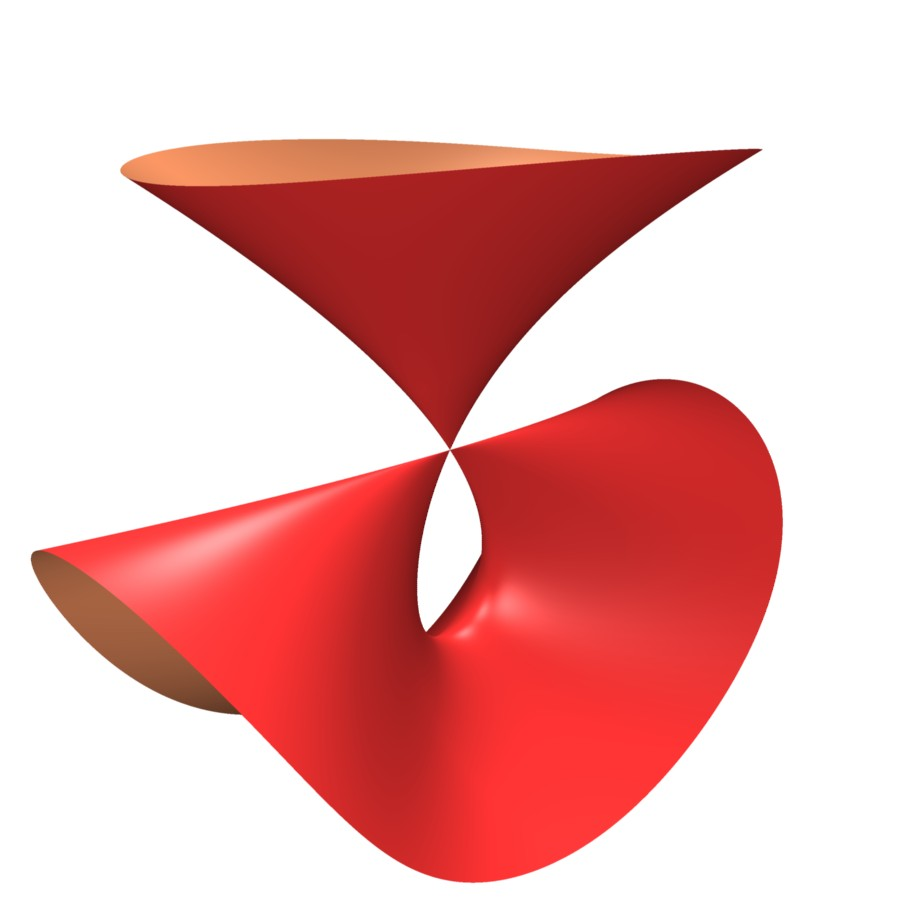
\includegraphics[width=1.1cm]{../../common/images/D5pm_03}\quad%
		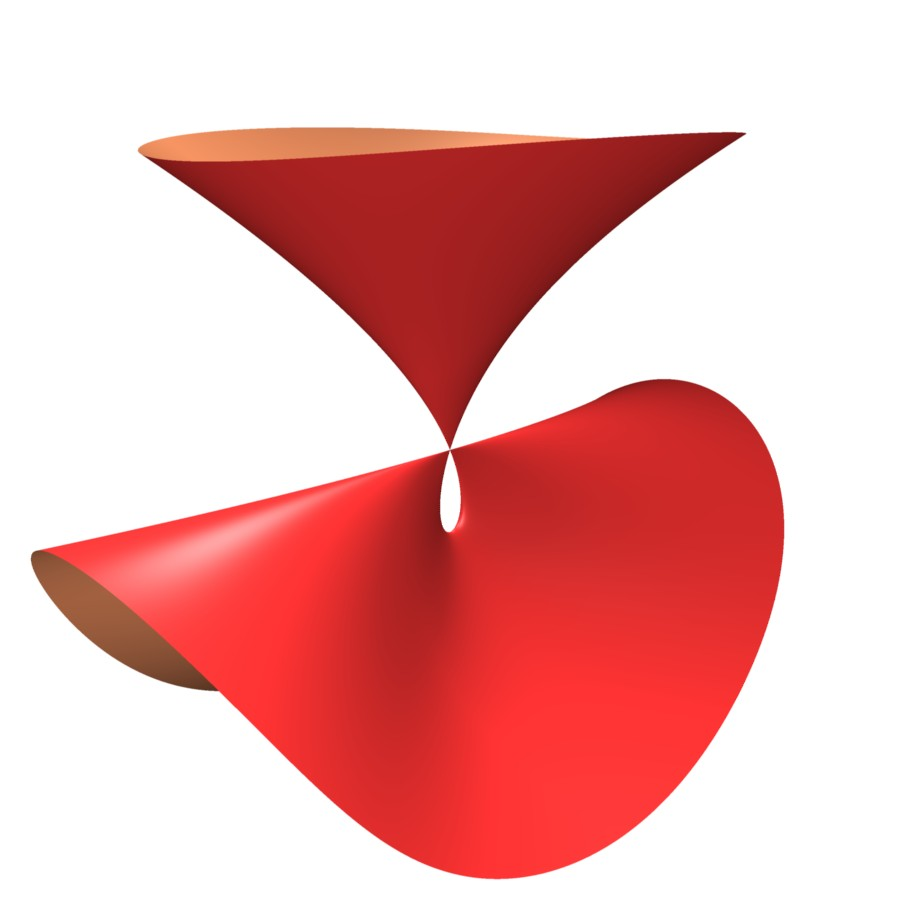
\includegraphics[width=1.1cm]{../../common/images/D5pm_02}\quad%
		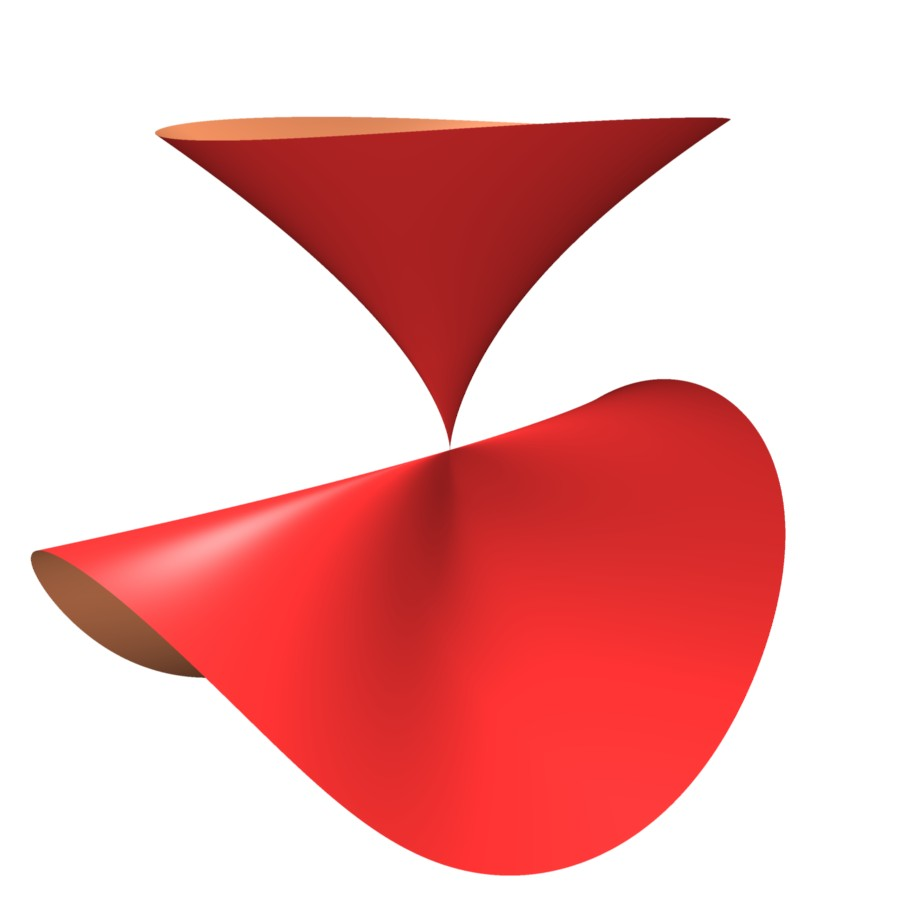
\includegraphics[width=1.1cm]{../../common/images/D5pm_01}%
	\end{Centering*}
	Alternatively, one can move the mountain up while keeping the position of the apex of the rock. This causes the rock to split into a real (visible) and an imaginary (invisible) part.
	\begin{Centering*}%
		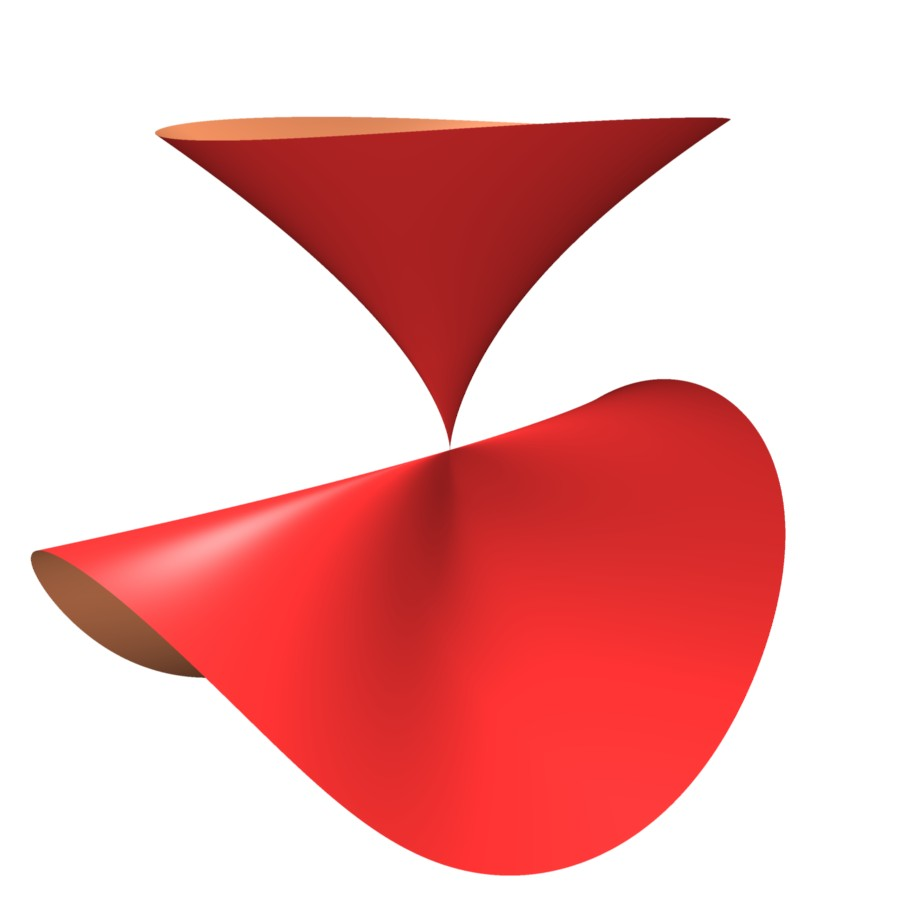
\includegraphics[width=1.1cm]{../../common/images/D5pm_01}\quad%
		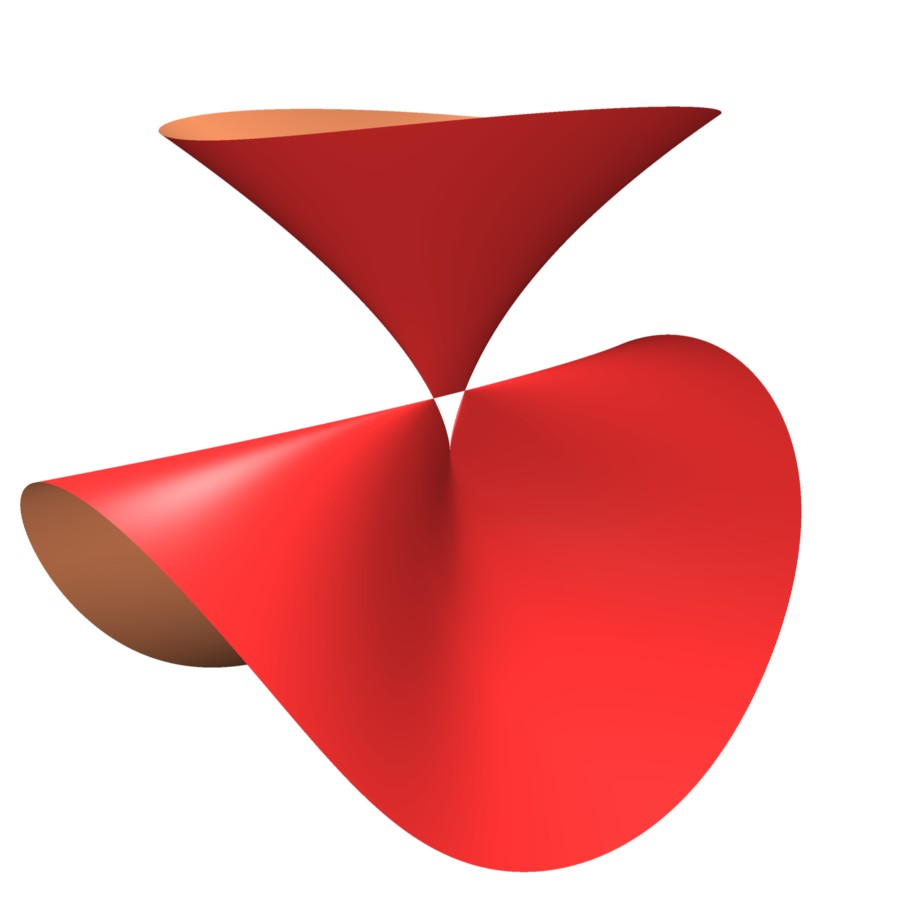
\includegraphics[width=1.1cm]{../../common/images/D5pm_04}\quad%
		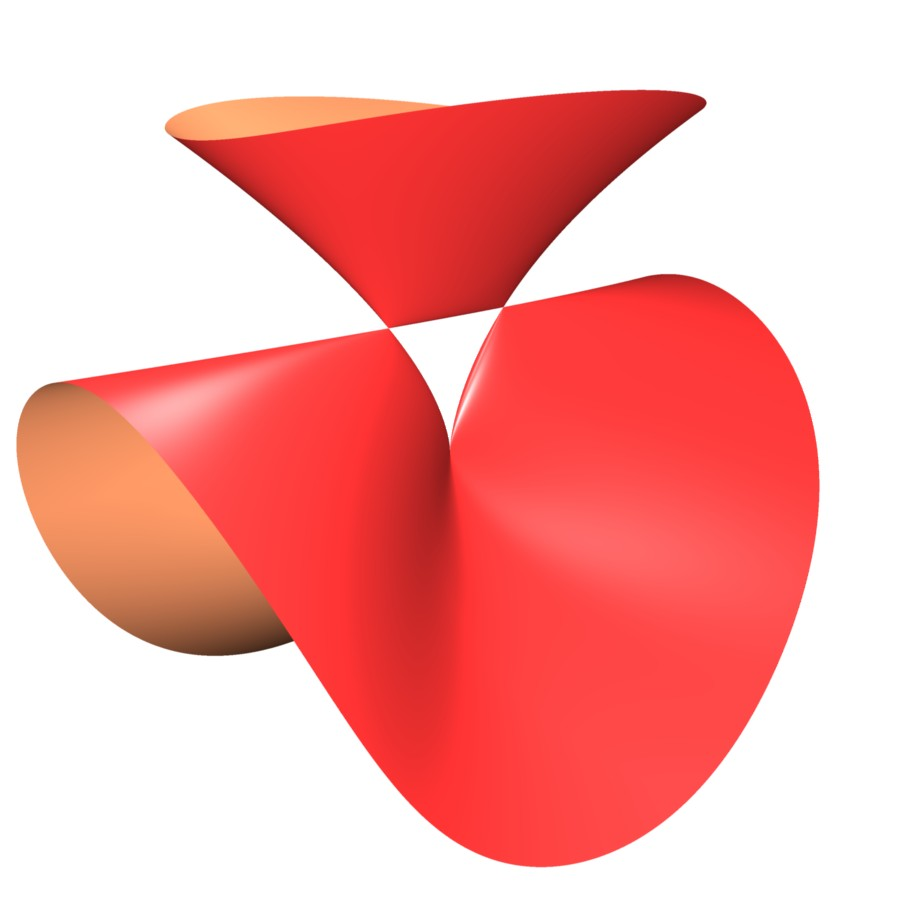
\includegraphics[width=1.1cm]{../../common/images/D5pm_05}%
	\end{Centering*}
\end{surferPage}
